\documentclass[10.5pt]{config}
% 本实验报告采用 署名-相同方式共享 4.0 国际许可协议 (CC BY-SA 4.0)
\usepackage{multirow}
\usepackage{wrapfig}
\usepackage{setspace}
\usepackage{titlesec}
\usepackage{ctex}
\usepackage{graphicx} % 用于插入图片
\usepackage{float}    % 用于控制图片位置
\usepackage{makecell}
\usepackage{tikz}
\usetikzlibrary{arrows.meta}

\titleformat{\subsubsection}[block]  % 设置为块级标题（自动换行）
{\normalfont\bfseries}{\thesubsubsection}{1em}{} 
\titlespacing*{\subsubsection}{1.5em}{3.25ex}{1.5ex}  % 调整缩进：左缩进2em
\setstretch{1.5}

% --- 请在这里填写您的个人信息 ---
\major{} % 专业
\name{}
\partner{} % 签名栏
\stuid{}
\date{} % 已更新为当前日期，可按需修改
\lab{}
\grades{}
\course{电工电子学实验}
\instructor{} % 指导老师
\exptype{基础实验} % 实验类型
\expname{晶体管共射放大电路} % 实验名字


\begin{document}

\makeheader % 首页头部

\section{实验目的}

\begin{enumerate}[label=\arabic*., leftmargin=2em]
    \item 掌握晶体管共射放大电路静态工作点的调整及测量方法，了解元件参数对静态工作点的影响。
    \item 掌握晶体管共射放大电路电压放大倍数、输入电阻、输出电阻等动态指标的测量方法。
    \item 熟悉双踪数字示波器和函数信号发生器的使用。
\end{enumerate}

\section{实验原理}

\begin{figure}[H] % h:当前位置, t:顶部, b:底部, p:独立一页
    \centering % 使图片居中
    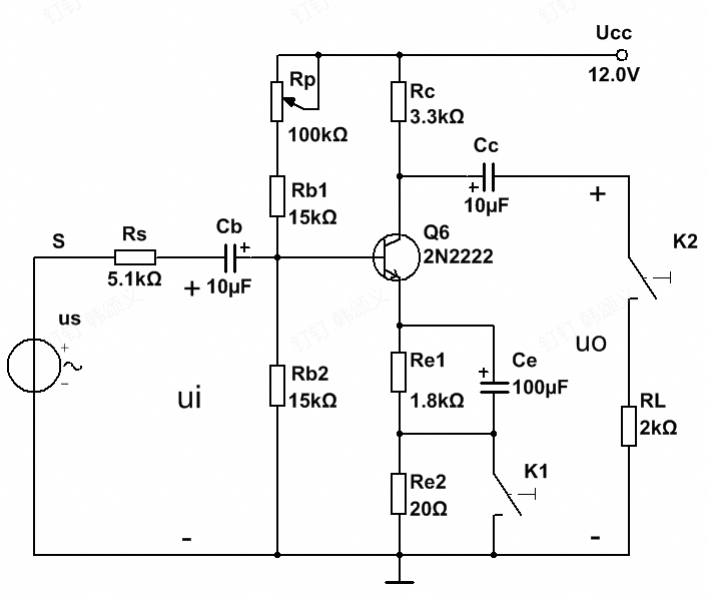
\includegraphics[width=0.5\textwidth]{figures/dianlu.png} % 插入图片并设置宽度
    \caption{实验电路图} % 图片下方的文字说明
    \label{fig:dianlu} % 用于文中引用
\end{figure}

\subsection*{1. 静态工作点的测量方法}

\begin{itemize}[leftmargin=2em]
    \item \textbf{直接测量法：} 实验电路接入直流电源 $U_{CC}=12\mathrm{V}$。在 $u_S=0$ 时，用数字式万用表的直流电压挡测量晶体管 C、E 之间的电压 $U_{CE}$，用微安表测量基极电流 $I_B$，毫安表测量集电极电流 $I_C$。
    
    \item \textbf{间接测量法：} 用数字式万用表的直流电压挡测量晶体管集电极电压 $U_C$ 和发射极电压 $U_E$，再利用公式 $U_{CE} = U_C - U_E$ 计算 $U_{CE}$。在放大电路中，通常利用测量集电极电阻 $R_C$ 两端的电压降 $U_{R_C}$ 来计算出 $I_C$，再利用公式 $U_{CE} = U_{CC} - R_C I_C$ 计算 $U_{CE}$。
\end{itemize}

\subsection*{2. 放大电路动态指标及测量}

\begin{itemize}[leftmargin=2em]
    \item \textbf{电压放大倍数 $A_u$：} 
    在静态工作点合适及输出电压 $u_o$ 不失真的情况下，测得晶体管共射放大电路输入电压 $u_i$ 的有效值 $U_i$ 和输出电压 $u_o$ 的有效值 $U_o$，则电压放大倍数：
    \begin{equation*}
        A_u = \frac{U_o}{U_i}
    \end{equation*}

    \item \textbf{输入电阻 $r_i$：}
    晶体管共射放大电路的输入电阻 $r_i$ 是指从放大电路输入端看进去的交流等效电阻。实验中一般采用换算法测量，通过在信号源和放大电路之间串接一个 $R_S$ 值取样电阻，测出 $U_S$ 和 $U_i$，则输入电阻：
    \begin{equation*}
        r_i = \frac{U_i}{U_S - U_i} R_S
    \end{equation*}
    测试时要注意 $U_S$ 不应取得太大，以免晶体管工作在非线性区。

    \item \textbf{输出电阻 $r_o$：}
    输出电阻 $r_o$ 是指将输入信号源短路，从输出端向电路看进去的交流等效电阻。采用换算法测量时，在输入、输出波形不失真的前提下，测得放大电路在空载和接入负载电阻 $R_L$ 两种情况下的输出电压 $U_o'$ 和 $U_o$，则输出电阻：
    \begin{equation*}
        r_o = \left( \frac{U_o'}{U_o} - 1 \right) R_L
    \end{equation*}
\end{itemize}

\subsection*{3. 静态工作点与波形失真}

在放大电路中，静态工作点的设置将直接影响电路是否能正常工作。
\begin{itemize}[leftmargin=2em]
    \item 当静态工作点电流 $I_C$ 过小时，此时 $U_{CE}$ 靠近 $U_{CC}$，随输入信号幅度的增大，将首先出现\textbf{截止失真}（输出波形 $u_o$ 正半周失真）。
    \item 当静态工作点电流 $I_C$ 过大时，此时 $U_{CE}$ 靠近 $0\mathrm{V}$，随输入信号幅度的增大，将首先出现\textbf{饱和失真}（输出波形 $u_o$ 负半周失真）。
\end{itemize}
因此，在一定输入信号幅度下，为避免输出波形失真，设置静态工作点电流 $I_C$ 的大小要合适。


\begin{figure}[H] % h:当前位置, t:顶部, b:底部, p:独立一页
    \centering % 使图片居中
    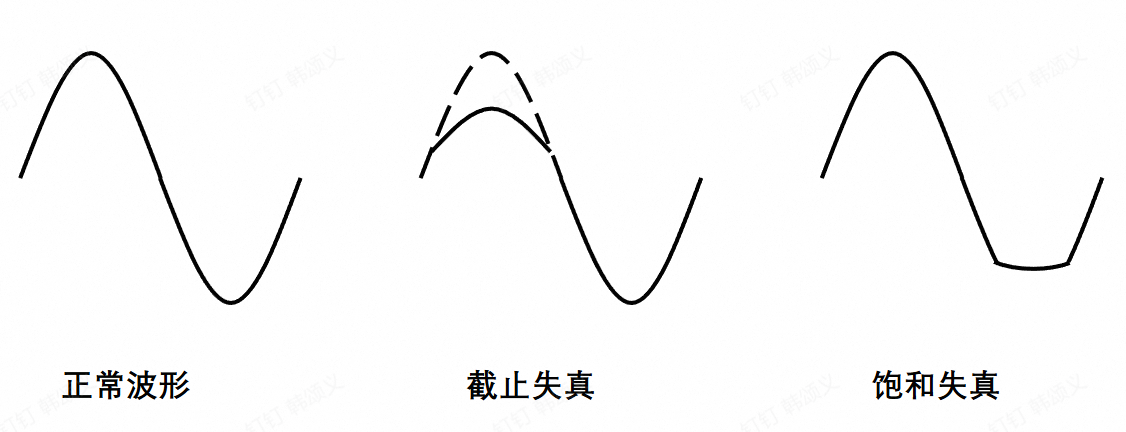
\includegraphics[width=0.35\textwidth]{figures/shizhen.png} % 插入图片并设置宽度
    \caption{失真示意图} % 图片下方的文字说明
    \label{fig:shizhen} % 用于文中引用
\end{figure}

\section{实验设备}
\begin{enumerate}[label=\arabic*., leftmargin=2em]
    \item 模拟电子技术实验箱
    \item 双踪数字示波器
    \item 函数信号发生器
    \item 数字式万用表
\end{enumerate}


\section{实验内容与步骤}

\begin{enumerate}[label=\arabic*., leftmargin=2em]
    \item \textbf{静态工作点的调整和测量：} 
    实验电路如图 \ref{fig:dianlu} 所示，接入 $U_{CC} = 12\mathrm{V}$ 直流电源。在 $u_S = 0$ 时，调节电位器 $R_P$，使放大电路的静态工作点满足 $I_C = 1.5\mathrm{mA}$。测量 $I_C$ 时，采用间接测量法，用万用表监控 $U_{R_C} = I_C R_C$。用万用表测量晶体管 T 的集电极电压 $U_C$、基极电压 $U_B$ 和发射极电压 $U_E$，并将数据记录入表 \ref{tab:static_point}。
    
    \item \textbf{电压放大倍数 $A_u$、输入电阻 $r_i$、输出电阻 $r_o$ 的测量：} 
    函数信号发生器输出 $u_S$ 为频率等于 $1\mathrm{kHz}$ 的正弦波信号，调节 $u_S$ 的幅度，使 $U_i = 10\mathrm{mV}$（有效值）。在输入 $u_i$、输出 $u_o$ 波形不失真的情况下，用示波器测量记录空载时的 $U_S$、$U_o'$ 和接入负载 $R_L$ 时的 $U_S$、$U_o$。数据记录到表 \ref{tab:dynamic_params}。

    \item \textbf{静态工作点对放大电路波形失真的影响：}
    保持电路为空载状态。在 $u_S = 0$ 时，调节 $R_P$，使 $I_C$ 的值过大或过小，用万用表测量 $U_C$、$U_E$、$U_{CE}$，计算 $I_C$。分别在 $I_C$ 的值过大、过小两种状态下，函数信号发生器输出 $u_S$ 为频率等于 $1kHz$ 的正弦波信号，逐渐增大输入信号幅度，使电路输出波形 $u_o$ 的底部或顶部出现明显失真。用示波器监视放大电路的输入波形 $u_i$ 和输出波形 $u_o$，测得 $u_i$ 的有效值 $U_i$。在表 \ref{tab:distortion} 中记录数据并判断波形的失真情况（饱和失真或截止失真）。
    
    \item \textbf{放大电路电压传输特性曲线的测量：}
    保持电路为空载状态。调节 $R_P$，使放大电路的静态工作点满足 $I_C = 1.5\mathrm{mA}$。函数信号发生器输出 $u_S$ 为频率等于 $1\mathrm{kHz}$ 的正弦波信号。用示波器同时观察整个电路的输入 $u_S$ 和输出 $u_o$ 的波形，调节 $u_S$ 的幅度，使得 $u_o$ 同时出现饱和失真和截止失真。采用示波器 XY 显示模式观察整个电路的电压传输特性曲线，并记录。
\end{enumerate}


\section{实验数据记录和处理}


\subsection{静态工作点的测量}

实际测量得到直流电源输出电压为$U = 12.0613V$.

\begin{table}[H]
    \centering
    \caption{静态工作点的测量}
    \label{tab:static_point}
    \begin{tabular}{|c|c|c|c|c|}
        \hline
        给定值 & \multicolumn{3}{c|}{测量值} & 计算值 \\ \hline
        $I_C / \mathrm{mA}$ & $U_C / \mathrm{V}$ & $U_B / \mathrm{V}$ & $U_E / \mathrm{V}$ & $U_{CE} / \mathrm{V}$ \\ \hline
        1.5 & 7.0996 & 3.3625 & 2.7238 & 4.3758 \\ \hline
    \end{tabular}
\end{table}

\subsection{电压放大倍数、输入电阻、输出电阻的测量}

\begin{table}[H]
    \centering
    \caption{电压放大倍数、输入电阻、输出电阻的测量}
    \label{tab:dynamic_params}
    \resizebox{\textwidth}{!}{
    \begin{tabular}{|c|c|c|c|c|c|c|c|c|}
        \hline
        $R_L / \mathrm{k}\Omega$ & $R_S / \mathrm{k}\Omega$ & $U_S / \mathrm{mV}$ & $U_i / \mathrm{mV}$ & $U_o' / \mathrm{mV}$ & $U_o / \mathrm{mV}$ & $A_u$ (计算) & $r_i / \mathrm{k}\Omega$ (计算) & $r_o / \mathrm{k}\Omega$ (计算) \\ \hline
        $\infty$ & \multirow{2}{*}{5.1} & 20.774 & \multirow{2}{*}{10} & 799.01 & / & 79.90 & 4.73 & \multirow{2}{*}{3.23} \\ \cline{1-1}\cline{3-3}\cline{5-8}
        2 & & 20.876 & & / & 305.27 & 30.53 & 4.69 & \\ \hline
    \end{tabular}
    }
\end{table}

\subsection{静态工作点对放大电路波形失真的影响}

\begin{table}[H]
    \centering
    \caption{静态工作点对放大电路波形失真的影响}
    \label{tab:distortion}
    \begin{tabular}{|c|c|c|c|c|c|c|}
        \hline
        $I_C / \mathrm{mA}$ (计算) & $U_C / \mathrm{V}$ & $U_E / \mathrm{V}$ & $U_{CE} / \mathrm{V}$ & $U_i / \mathrm{mV}$ & 失真情况 \\ \hline
        1 & 8.7931 & 1.85491 & 6.9382 & 35.703 & 截止失真 \\ \hline
        2 & 5.6526 & 3.5352 & 2.1174 & 14.376 & 饱和失真 \\ \hline
    \end{tabular}
\end{table}

\begin{figure}[H] % h:当前位置, t:顶部, b:底部, p:独立一页
    \centering % 使图片居中
    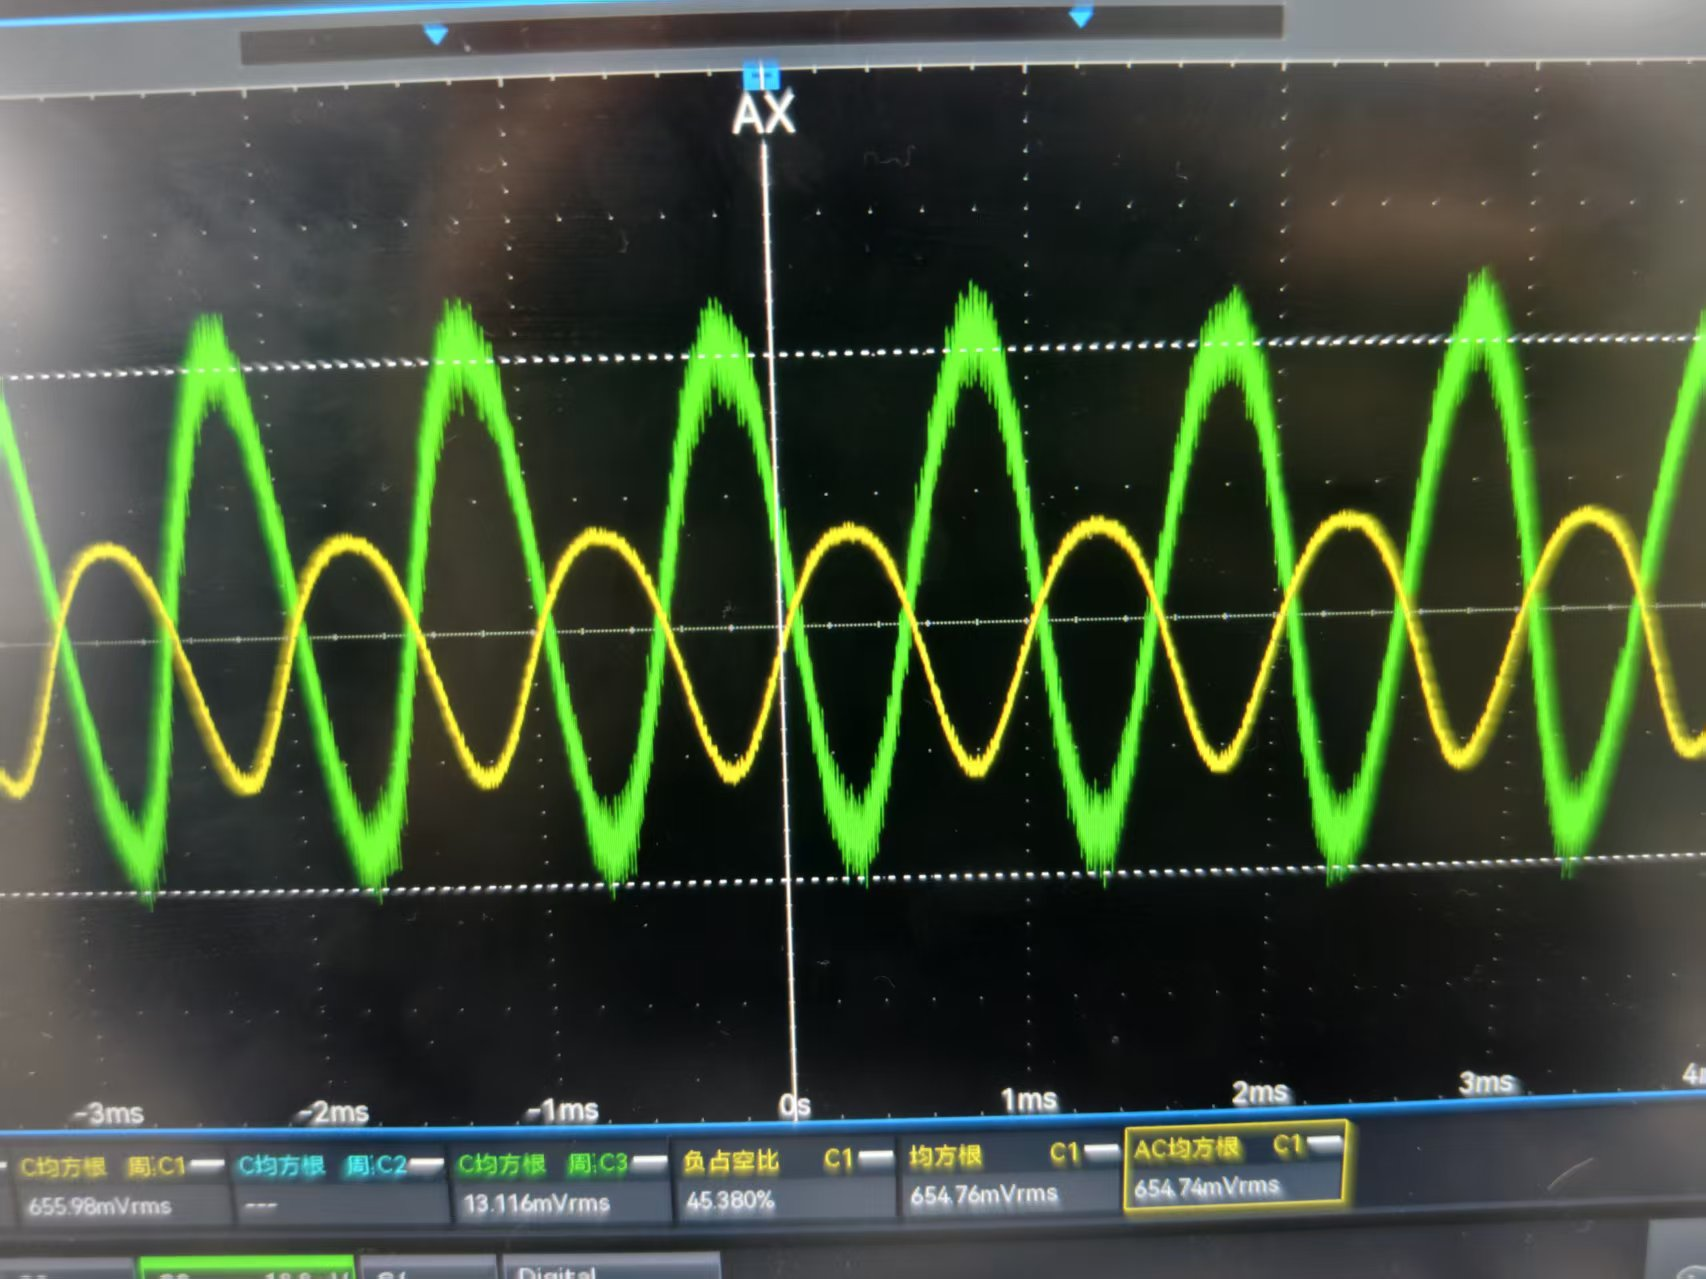
\includegraphics[width=0.4\textwidth]{figures/jiezhi.jpg} % 插入图片并设置宽度
    \caption{截止失真波形} % 图片下方的文字说明
    \label{fig:jiezhi} % 用于文中引用
\end{figure}

\begin{figure}[H] % h:当前位置, t:顶部, b:底部, p:独立一页
    \centering % 使图片居中
    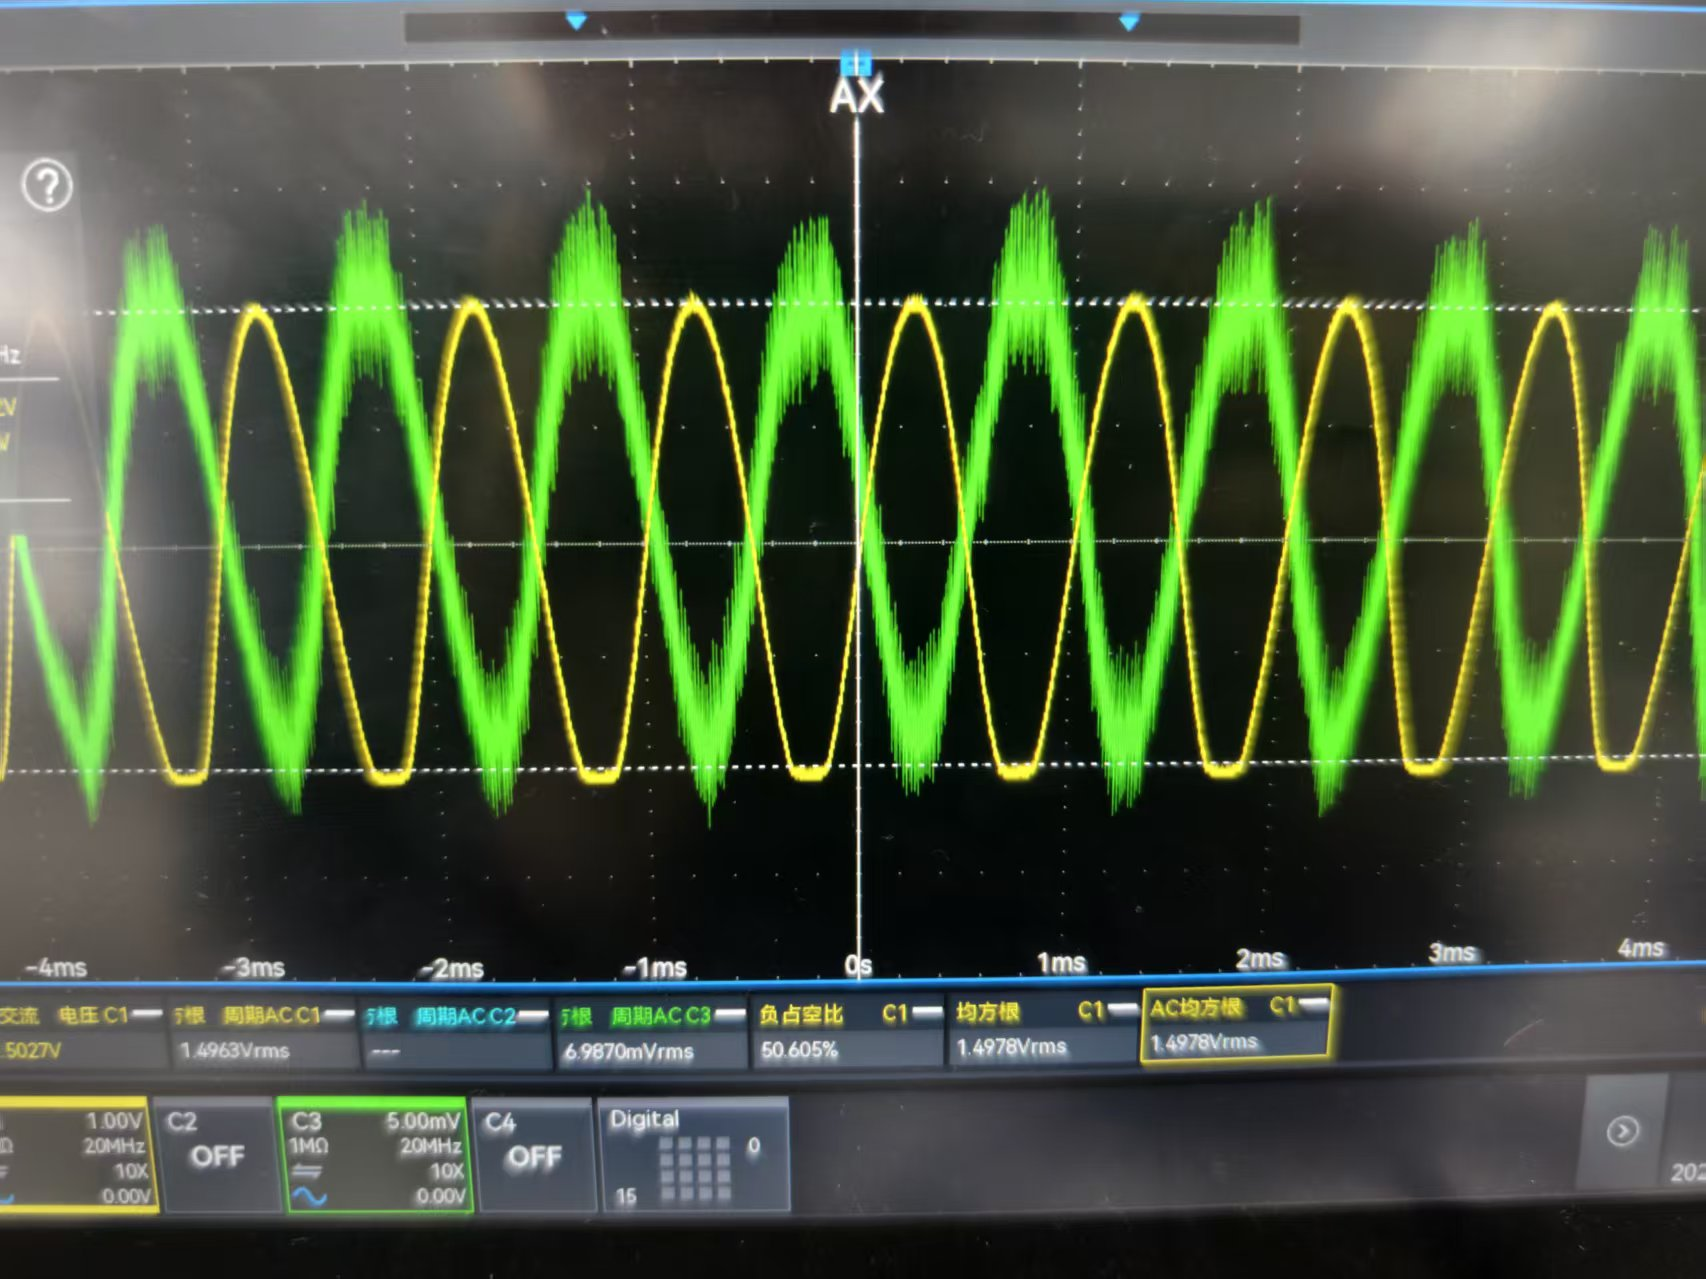
\includegraphics[width=0.4\textwidth]{figures/baohe.jpg} % 插入图片并设置宽度
    \caption{饱和失真波形} % 图片下方的文字说明
    \label{fig:baohe} % 用于文中引用
\end{figure}

\subsection{放大电路电压传输特性曲线测量}

\begin{figure}[H] % h:当前位置, t:顶部, b:底部, p:独立一页
    \centering % 使图片居中
    
\includegraphics[width=0.4\textwidth]{figures/xy.jpg} % 插入图片并设置宽度
    \caption{电压传输特性曲线} % 图片下方的文字说明
    \label{fig:xy} % 用于文中引用
\end{figure}


\section{实验结果与分析}

\subsection*{1. 静态工作点分析}
根据表 \ref{tab:static_point} 测得的数据，在给定 $I_C = 1.5\mathrm{mA}$ 时：
\begin{itemize}[leftmargin=2em]
    \item 晶体管的发射结偏置电压 $U_{BE} = U_B - U_E = 3.3625\mathrm{V} - 2.7238\mathrm{V} \approx 0.64\mathrm{V}$，符合硅晶体管正向导通的压降特征。
    \item 集电结电压 $U_{BC} = U_B - U_C = 3.3625\mathrm{V} - 7.0996\mathrm{V} < 0$，集电结处于反向偏置状态。
\end{itemize}
发射结正偏、集电结反偏，说明晶体管正常工作在\textbf{放大区}。同时，$U_{CE} = 4.3758\mathrm{V}$，处于电源电压 ($12\mathrm{V}$) 的适中位置，说明该静态工作点设置较为合理，能够为交流信号提供较大的动态范围。

\subsection*{2. 动态指标（放大倍数与输入/输出电阻）分析}
由表 \ref{tab:dynamic_params} 的数据计算可知：
\begin{itemize}[leftmargin=2em]
    \item \textbf{电压放大倍数：} 空载时电压放大倍数 $A_{u1} \approx 79.90$，而接入 $2\mathrm{k}\Omega$ 负载后，放大倍数锐减至 $A_{u2} \approx 30.53$。这直观地反映了共射放大电路的带负载能力有限。
    \item \textbf{输出电阻：} 计算得 $r_o \approx 3.23\mathrm{k}\Omega$。由于放大电路本身存在输出电阻 $r_o$，当接入负载 $R_L$ 时，$r_o$ 会与 $R_L$ 形成分压效应，从而导致实际输出电压 $U_o$ 远低于空载输出电压 $U_o'$。
    \item \textbf{输入电阻：} 计算得 $r_i \approx 4.7\mathrm{k}\Omega$，验证了共射放大电路具有中等输入电阻的理论特性。
\end{itemize}

\subsection*{3. 静态工作点对波形失真的影响分析}
结合表 \ref{tab:distortion} 及图 \ref{fig:jiezhi}、图 \ref{fig:baohe} 所示波形：
\begin{itemize}[leftmargin=2em]
    \item \textbf{截止失真：} 当静态偏置电流减小至 $I_C = 1\mathrm{mA}$ 时，$U_{CE}$ 偏高 ($6.9382\mathrm{V}$)，工作点靠近截止区。此时增大输入信号，交流信号的负半周会使基极电流减小至 0 以下，晶体管进入截止状态。由于共射电路反相输出，导致输出电压 $u_o$ 的\textbf{顶部被削平}。
    \item \textbf{饱和失真：} 当静态偏置电流增大至 $I_C = 2\mathrm{mA}$ 时，$U_C$ 降低，$U_{CE}$ 减小至 $2.1174\mathrm{V}$，工作点靠近饱和区。此时增大输入信号，交流信号的正半周会导致集电极电流过大，晶体管进入饱和状态，$U_{CE}$ 无法继续下降，导致输出电压 $u_o$ 的\textbf{底部被削平}。
\end{itemize}
实验结果与理论完全吻合，证明了静态工作点的位置直接决定了放大电路不失真输出的最大动态范围。

\subsection*{4. 电压传输特性曲线分析}
从示波器 XY 模式观察并记录的电压传输特性曲线（图 \ref{fig:xy}）可以看出，曲线中间部分为一条斜率较大的近似直线，该区域即为晶体管的\textbf{线性放大区}，其斜率大小反映了电压放大倍数。曲线两端趋于平缓：左侧平缓区对应晶体管的截止区（输出高电平），右侧平缓区对应晶体管的饱和区（输出低电平），直观地展示了晶体管的非线性特征及其动态工作区间。


\section{讨论、心得}

本次晶体管共射放大电路实验，将课堂上抽象的理论知识与实际的硬件电路紧密结合，让我对模拟电子技术有了更直观、更深刻的理解。以下是我的几点心得体会：

\begin{itemize}[leftmargin=2em]
    \item 实验中最令我印象深刻的是静态工作点（Q点）对整个放大电路性能的决定性作用。在调节电位器改变 $I_C$ 的过程中，我直观地观察到了输出波形从完整到顶部削平（截止失真）、再到底部削平（饱和失真）的动态演变。这让我深刻认识到，合适的直流偏置是交流信号能够实现最大不失真放大的先决条件。
    
    \item 在测量动态指标时，空载与带载状态下输出电压的巨大差异（$799.01\mathrm{mV}$ 骤降至 $305.27\mathrm{mV}$），让我真切地感受到了放大电路本身输出电阻 $r_o$ 的存在及其带来的“分压”效应。这不仅验证了理论公式，也让我意识到了在未来的实际工程应用中，必须充分考虑电路的带载能力和前后级的级联匹配问题。
\end{itemize}

总的来说，这次实验不仅巩固了我的电路分析基础，更增强了我的动手实践和故障排查能力，为后续更复杂的硬件控制系统和电子设计打下了很好的基础。

\end{document}